\documentclass[english,dvipdfmx]{jsarticle}
\usepackage{amsmath,amssymb}
\usepackage{color}
\usepackage[hiresbb]{graphicx}
\usepackage{here}
\newcommand{\average}[1]{\ensuremath{\langle#1\rangle} }
\newcommand*{\point}{\textcircled{\textcolor{red}{\scriptsize キ}}}
\newcommand*{\proof}{\textcircled{\textcolor{blue}{\scriptsize P}}}
\begin{document}
\section{二項関係}
\begin{description}
    \item[\bf{Definition:}] 集合$X$上の同値関係 $R \subset X \times X$ \\
    \point : 等号関係の一般化
    \begin{equation*} \begin{cases}
        \text{反射律} : \quad &xRx \quad ( \forall x \in X )  \\
        \text{対称律} : \quad  &xRy \Rightarrow yRx \quad ( \forall x,y \in X ) \\
        \text{推移律} : \quad &xRy , yRz \Rightarrow xRz \quad (\forall x,y,z \in X )
    \end{cases} 
    \end{equation*}
    \item[\bf{Example:}] 同値関係の例 $R$
    \begin{enumerate}
        \item $ = $
        \item 合同, 相似 (幾何)
        \item $x \equiv y \quad (mod \ p)$
    \end{enumerate} 
    \item[\bf{Definition:}] 同値類
    \begin{equation*}  
        [a] = \{ x \in X \ | \ xRa \} \quad ( a \in X , R : \text{relation on a set } X )
    \end{equation*}
    \item[\bf{Definition:}] 商集合 \\
    \textcircled{\textcolor{red}{\scriptsize キ}} : 同値類集合の集合
    \begin{equation*} 
    X / R = \{ [a] \ | \ a \in X \} 
    \end{equation*}
    \item[\bf{Definition:}] 自然な射影
    \begin{equation*} 
    \gamma : X \longmapsto X / R ,\ \gamma(x) = [x] \quad ( x \in X )
    \end{equation*}
    \item[\bf{Definition:}] 集合$X$上の\textcolor{red}{順序}関係 $R \subset X \times X \ ( xRy \Leftrightarrow x\leq y)$ \\ 
    \point : 大小関係の一般化
    \begin{equation*}
    \begin{cases}
        \text{反射律} : \quad &x\leq x \quad ( \forall x \in X )  \\
        \text{\color{red} 反対称律} : \quad  &x\leq y ,y\leq x \Rightarrow x=y \quad ( \forall x,y \in X ) \\
        \text{推移律} : \quad &x\leq y , y\leq z \Rightarrow x\leq z \quad (\forall x,y,z \in X )
    \end{cases}
    \end{equation*}
    \item[\bf{Definition:}] 順序集合$(X , \leq)$ \\
        $\leq$ は$X$上の順序関係.
    \item[\bf{Example:}] 順序集合の例
    \begin{enumerate}
        \item $ (\mathbb{R},\leq) $ は順序集合, $ (\mathbb{R},<) $ は順序集合でない.
        \item $ ( 2^X,\subset) $
    \end{enumerate}
    \item[\bf{Definition:}] 順序部分集合 $(M,\leq_M) \subset (X, \leq)$
    \begin{equation*} 
        M \subset X , a \leq_M b \Leftrightarrow a \leq b
    \end{equation*}
    \item[\bf{Definition:}] 半順序, 全順序
    \begin{eqnarray*} 
        \exists (x,y) \in R \quad ( x,y \in X ) &\Rightarrow& R \text{ is partial order} ,\ (X , R) \text{ is partially ordered set} \\
        \forall (x,y) \in R \quad ( x,y \in X ) &\Rightarrow& R \text{ is total order} ,\ (X , R) \text{ is totally ordered set}
    \end{eqnarray*}
\end{description}
\newpage
\section{半順序集合}
\begin{description}
    \item[\bf{Definition:}] 最大値 (最小値) , 上限 (下限) and 上界 (下界)
    \begin{eqnarray*}
    \max \ A = {\color{red}M}  &\Leftrightarrow& a \leq {\color{red}M} \quad ( {\color{red}M} \in A ,\ \forall a \in A )  \\
    {\color{red}{s}} \text{ is one of upper bounds of } A &\Leftrightarrow& a \leq {\color{red}{s}} \quad ( \forall a \in A ) \\
    \sup \ A = {\color{red}M'} &\Leftrightarrow& \min \ S = {\color{red}M'} \quad ( S \text{ is a set of upper bounds of }A ) \\
    &\Leftrightarrow& \begin{cases}  \forall a \in A  ,\ a \leq {\color{red}M'} \\ \forall \epsilon > 0 ,\ \exists a \in A \ \text{s.t.} \ {\color{red}M'} - \epsilon < a \end{cases}
    \end{eqnarray*}
    \item[\bf{Example:}] 半順序集合の例 $ \{ y \} \leq \{ x,z \} $ の順序は定義されていない. \\
        \begin{minipage}{.4\textwidth}
            \centering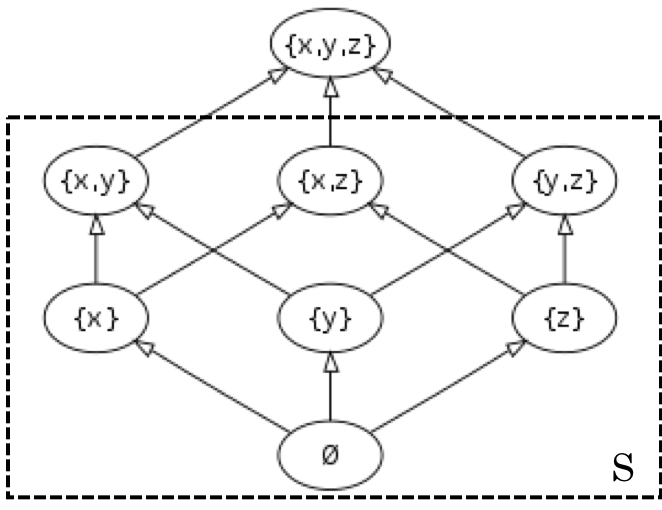
\includegraphics[width=7cm]{./set.png}
            \end{minipage}
            \hfill
            \begin{minipage}{.4\textwidth}
        $\max \ S$ : $None$ , $\min \ S$ : $\phi$\\
        $\sup \ S$ : $\{ x,\ y,\ z \}$ , $\inf \ S$ : $\phi$
        \end{minipage}
    \item[\bf{Theorem:}] 最大値, 最小値, 極大値 , 極小値 は一意に存在する.\\
        \proof : 最大値, 最小値の一意性は順序関係の反対称律を使う. \\
        \proof : 極大値, 極小値の一意性は最大値,最小値の一意性を使う.
    \item[\bf{Theorem:}] 集合 $A$ に最大(最小)値が存在するならば, $\max \ A = \sup \ A$ ($\min \ A = \inf \ A$ ). \\
        \proof : $\sup(\inf)$ の2つめの定義を使う.
    \item[\bf{Axiom:}] 上限と下限の存在(実数の連続性)
        \begin{equation*} 
            A \subset \mathbb{R},\ A \neq \phi,\ 
            \begin{cases}
            A\text{が上に有界} \Rightarrow \sup A \in \mathbb{R} \text{が存在}  \\
            A\text{が下に有界} \Rightarrow \inf A \in \mathbb{R} \text{が存在}
            \end{cases} 
        \end{equation*}
    \item[\bf{Definition:}] 完備束 \\
        半順序集合 $X$, $\forall X' \subset X,\ \exists \sup \ X',\ \inf \ X'.$
\end{description}
\newpage
\section{点列}
    \begin{description}
        \item[\bf{Definition:}] 点列は写像 $ x : \mathbb{N} \longmapsto X $である.
        \item[\bf{Definition:}] 部分点列は合成写像 $ x \circ \iota : \mathbb{N} \longmapsto X$ \\
        ただし, $\iota : \mathbb{N} \longmapsto \mathbb{N} $ は $ i \leq j \Rightarrow \iota(i) \leq \iota(j) $を満たす.
        \item[\bf{Example:}] 点列と部分点列の概要
            \begin{figure}[H]
                \begin{center}
                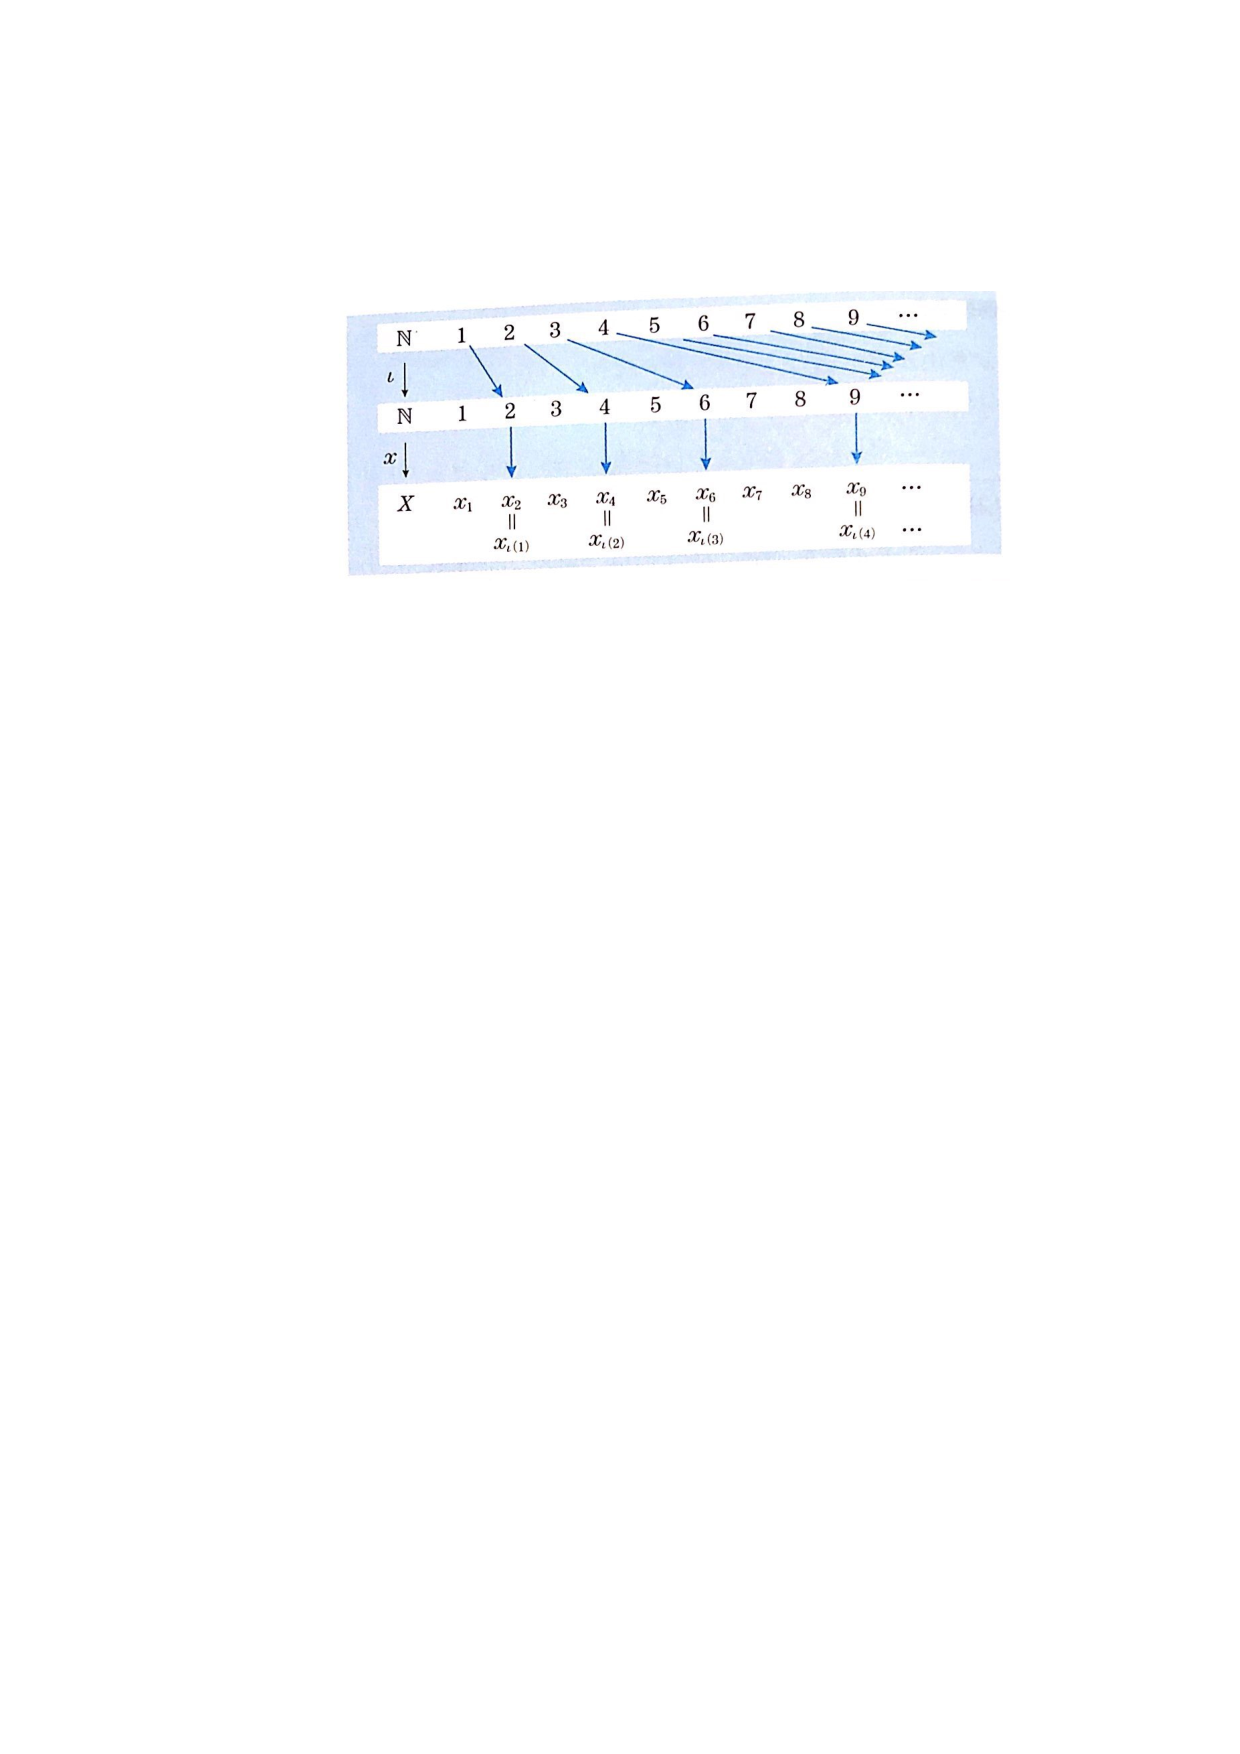
\includegraphics[clip,width=10cm]{./sequence.pdf}
                \caption{点列}
                \end{center}
            \end{figure}
        \item[\bf{Definition:}] 点列の極限 \\
            $\alpha$ は点列の極限値である. $\Leftrightarrow$
            \begin{equation*}
                \forall \epsilon > 0 ,\ \exists N \in \mathbb{N} \text{ s.t. } n \geq N \Rightarrow | x_n - \alpha | < \epsilon
            \end{equation*}
        \item[\bf{Theorem:}] 数列$(a_n)$が拡大実数系に極限をもつとき, その部分列の極限と一致する. \\
            \point : 元の数列が振動する場合などは, 部分列極限は複数存在する.
        \item[\bf{Definition:}] 上極限, 下極限 \\
            
        \item[\bf{Definition:}] 上に有界, 下に有界 \\
            点列 $\{ x_n \}$  は上に有界である. $\Leftrightarrow$
            \begin{equation*}
                \exists M \in \mathbb{R},\ \forall i \in \mathbb{N},\ x_i \leq M
            \end{equation*}

        \item[\bf{Definition:}] Cauchy列 \\
            \point : 十分大きな$N \in \mathbb{N}$を選ぶと$n,\ m \geq N$において$x_n$と$x_m$の差をいくらでも小さくできる列. \\
            $\{ x_n \}$ がCauchy列である. $\Leftrightarrow$
            \begin{equation*}
                \forall \epsilon > 0,\ \exists N \in \mathbb{N} \text{ s.t. } n,\ m \geq N \Rightarrow | x_n - x_m | < \epsilon
            \end{equation*}
        \item[\bf{Example:}] Cauchy列の例 \\
            %% TODO Cauchy Sequence の 例 を書く. 証明をすること.
        \item[\bf{Theorem:}] $\{ x_n \} ,\ \{ y_n \}$ がCauchy列 $\Rightarrow$
            \begin{equation*}
                \{ x_n + y_n \} ,\ \{ x_n \cdot y_n \} \text{ はCauchy列.} 
            \end{equation*}
        \item[\bf{Theorem:}] 点列 $x_n$ が収束する $\Rightarrow$ $x_n$ はCauchy列.
        \item[\bf{Theorem:}] 点列 $x_n$ がCauchy列 $\Rightarrow$ $x_n$ は有界.
        
    \end{description}

\newpage
\section{実数}
    \subsection{$\mathbb{N}$ の定義と $\mathbb{Z},\ \mathbb{Q}$ の構成}
    \begin{description}
        \item[\bf{Axiom:}] ペアノの公理 \\
        \point : 自然数の定義 \\
        後者を与える関数 $S$ を定義する. (ex. $S(1) = 2$ )
        \begin{enumerate}
            \item $0$ は自然数.
            \item 全ての自然数 $n$に対し, $S(n)$ は自然数.
            \item 全ての自然数 $n$に対し, $S(n) = 0$ とならない.
            \item $a,\ b \in \mathbb{N},\ a \neq b \Rightarrow S(a) \neq S(b)$
            \item $\Phi$ を単項述語関数とする.
                \begin{itemize}
                    \item $\Phi(0)$ が真.
                    \item 全ての自然数 $n$ に対し, $\Phi(n)$ が真ならば $\Phi(S(n))$ は真.
                \end{itemize}
                ( \bf{数学的帰納法} )
        \end{enumerate}
        \item[\bf{Definition:}] 整数と有理数
            \begin{equation*}  
            \mathbb{Z} = \mathbb{N} \cup -\mathbb{N} ,\ \mathbb{Q} = \{ \frac{b}{a} \mid a,\ b \in \mathbb{Z},\ a \neq 0 \}
            \end{equation*}
    \end{description}
    \subsection{$\mathbb{R}$の構成}
    \subsubsection{デデキント切断}
    \begin{description}
    \item[\bf{Definition:}] $\mathbb{Q}$上のデデキント切断
        \begin{equation*}
            A \cup B = \mathbb{Q},\ A \cap B = \phi,\ A \neq \phi,\ B \neq \phi,\ a \in A,\ b \in B \Rightarrow a < b
        \end{equation*}
    \item[\bf{Definition:}] 実数 $\alpha$ をデデキント切断の境界値 $\alpha = \average{A \mid B}$ として定義する. \\
        \point : 有理数全体集合のデデキント切断の境界値を実数と定義.
    \end{description}
    \subsubsection{有理数のCauchy列を用いた完備化}
    \begin{description}
    \item[\bf{Definition:}] Cauchy列の同値関係
        \begin{eqnarray*}
            \{ a_n \} \sim \{ b_n \} &\Leftrightarrow& \lim_{n \to \infty} a_n = \lim_{n \to \infty} b_n = \alpha \\
            &\Leftrightarrow& \forall \epsilon > 0,\ \exists N \in \mathbb{N} \text{ s.t. } n \geq N \Rightarrow | a_n - b_n | < \epsilon
        \end{eqnarray*}
    \item[\bf{Definition:}] $\mathbb{R}$ \\
        全単射 $ \Phi : (S \ / \sim) \longmapsto \mathbb{R} \quad ( S \text{ is the set of all Cauchy Sequences on }\mathbb{Q} ) $ を定義.
        \begin{equation*}
            \Phi( [\{ a_n \}] ) = \lim_{n \to \infty} a_n \in \mathbb{R}
        \end{equation*}
        \point : $\mathbb{Q}$上のCauchy列の同値類と実数の間に1対1写像を定義する.
        \item[\bf{Example:}] ネイピア数 $e = \displaystyle \lim_{n \to \infty} ( 1 + \frac{1}{n} )^n ,\ a_n = (1 + \frac{1}{n})^n\text{ はCauchy列.}$ 
    \end{description}
    \subsection{実数の性質}
    \subsubsection{有理数の稠密性 / 無理数の稠密性}
        %% TODO 証明をきちんと追っておくこと.
        \begin{description}
            \item[\bf{Theorem:}] 有理数の稠密性 \\
                \point : 2つの実数の間に有理数が存在. 
                \begin{equation*}
                    \forall x,\ y \in \mathbb{R},\ x < y \Rightarrow \exists r \in \mathbb{Q} \text{  s.t. } x < r < y
                \end{equation*}
                ※ 他の表現 : $ \forall \epsilon > 0 ,\ a \in \mathbb{R} ,\ \exists r \in \mathbb{Q},\ | a - r | < \epsilon $
            \item[\bf{Theorem:}] 無理数の稠密性 \\
                \point : 2つの実数の間に無理数が存在. 
                \begin{equation*}
                    \forall x,\ y \in \mathbb{R},\ x < y \Rightarrow \exists q \in \mathbb{R} \backslash \mathbb{Q} \text{  s.t. } x < q < y
                \end{equation*}
            \item[\bf{Theorem:}] アルキメデスの性質(有理数の稠密性と同値)
                \begin{equation*}
                    \forall a,\ b \in \mathbb{R},\ 0 < a < b \Rightarrow \exists n \in \mathbb{N} \text{ s.t. } b < na
                \end{equation*}
            \item[\bf{Theorem:}] $\mathbb{N} \subset \mathbb{R}$ は上に有界でない. (有理数の稠密性と同値)
            \item[\bf{Theorem:}] $lim_{n \to \infty} \frac{1}{n} = 0$ (有理数の稠密性と同値)
        \end{description}
    \subsubsection{実数の完備性}
        \begin{description}
            \item[\bf{Axiom:}] $\mathbb{R}$ 上の全てのCauchy列は収束する. \\
            \point : 一般 : 収束列 $\Rightarrow$ Cauchy列, $\mathbb{R}$ : 収束列$\Leftrightarrow$ Cauchy列.
            \item[\bf{Axiom:}] カントールの区間縮小定理 \\
            
        \end{description}
    \subsubsection{実数の連続性}
    \point : 有理数の稠密性(4.3.1) \& 実数の完備性(4.3.2) と同値
    \begin{description}
        \item[\bf{Axiom:}] 実数の連続性 \\
            \begin{equation*} 
                A \subset \mathbb{R},\ A \neq \phi,\ 
                \begin{cases}
                A\text{が上に有界} \Rightarrow \sup A \in \mathbb{R} \text{が存在}  \\
                A\text{が下に有界} \Rightarrow \inf A \in \mathbb{R} \text{が存在}
                \end{cases} 
            \end{equation*}
        \item[\bf{Theorem:}] デデキントの定理(実数の連続性と同値)\\
            実数集合上の全ての切断 $\average{A \mid B}$ に対し,
            \begin{equation*}
                \alpha \in A ,\ \beta \in B \Rightarrow \exists \gamma \in \mathbb{R} \ s.t. \ \alpha \leq \gamma \leq \beta ,\ \gamma \text{ is } {\color{red}{\max A}} \text{ or } {\color{red}{\min B}}
            \end{equation*}
            ただし, $\mathbb{R}$ 上のデデキント切断は
            \begin{equation*}
                A \cup B = \mathbb{R},\ A \cap B = \phi,\ A \neq \phi,\ B \neq \phi,\ a \in A,\ b \in B \Rightarrow a < b
            \end{equation*}
            \point : $\mathbb{R}$の数直線を二つに切断するイメージ.

        \item[\bf{Theorem:}] 単調有界数列の収束定理(実数の連続性と同値) \\
            数列$(a_n)$が単調増加かつ上に有界ならば$(a_n)$は収束する. \\
            数列$(a_n)$が単調減少かつ下に有界ならば$(a_n)$は収束する.
        
        \item[\bf{Theorem:}] ボルツァーノ-ワイアシュトラウスの定理(実数の連続性と同値)\\
            任意の有界数列$(a_n)$が収束する部分列をもつ. \\
            以下の言い換えが可能.
            \begin{itemize}
                \item $A \subset \mathbb{R}$が点列コンパクト $\Leftrightarrow A$が有界閉集合.
                \item 距離化可能空間に置いてコンパクトと点列コンパクトは同値より, \\ 
                $A \subset \mathbb{R}$がコンパクト $\Leftrightarrow A$が有界閉集合. (ハイネボレルの定理)
            \end{itemize}
            

            
    
    \end{description}

\newpage
\section{濃度}
    \begin{description}
        \item[\bf{Definition:}] 集合 $A$ の濃度. $|A|,\ card \ A ,\ \# A $ etc...
            \begin{equation*}
                |A| = 
                \begin{cases}
                    \ n \in \{ 0 \} \cup \mathbb{N} &: \text{有限集合の濃度} \\
                    \ (others) &: \text{無限集合の濃度} \quad ex.
                    \begin{cases}
                        \ \aleph_0 &: \text{ 可算無限集合の濃度 } \\
                        \ \aleph &: \text{ 連続体の濃度 }
                    \end{cases}
                \end{cases}
            \end{equation*}
        \item[\bf{Definition:}] $|A| = |B| \Leftrightarrow A \sim B \Leftrightarrow \exists f \text{ (全単射) } : A \longmapsto B $ \\
            集合$S$上の同値関係$ R = \{ (A,B) \mid |A| = |B| \ \} \subset S \times S$
        \item[\bf{Definition:}] $|A| \leq |B|  \Leftrightarrow \exists f \text{ (単射) } : A \longmapsto B $ \\
            集合$S$上の順序関係$ R = \{ (A,B) \mid |A| \leq |B|  \} \subset S \times S$ \\
            \proof : 反対称律はBernsteinの定理を用いる.
        \item[\bf{Theorem:}] $ \aleph_0 < \aleph $ \\
            \proof : $ \mathbb{N} \not\sim  [ 0, 1 )$ をカントールの対角線論法で示す.
        \item[\bf{Theorem:}] $ |X| < |\mathfrak{P}(X)| $ \\
            \proof : $X \subset \mathfrak{P}(X)$より, $|X| \leq |\mathfrak{P}(X)|$は明らか.$|X| \not= |\mathfrak{P}(X)|$を対角線論法で示す.
        \item[\bf{Theorem:}] $A \cap B = \phi$ とする.
            \begin{enumerate}
                \item $\cup$
                    \begin{equation*}
                        | A \cup B | = | A | + | B | 
                    \end{equation*}
                    \begin{table}[H]
                        \begin{center}
                        \begin{tabular}{|c|c|c|c|} \hline
                            $|A \cup B| $& 有限 & 可算 & 非可算 \\ \hline
                            有限 & 有限 &  可算 & 非可算 \\ \hline
                            可算 &  & 可算 & 非可算 \\ \hline
                            非可算 & & & 非可算 \\ \hline
                        \end{tabular}
                    \end{center}
                    \end{table}
                \item $\times$
                    \begin{equation*}
                        | A \times B | = | A | \cdot | B | 
                    \end{equation*}
                    \begin{table}[H]
                        \begin{center}
                        \begin{tabular}{|c|c|c|c|} \hline
                            $|A \times B| $& 有限 & 可算 & 非可算 \\ \hline
                            有限 & 有限 & 可算 & 非可算 \\ \hline
                            可算 &  & 可算 & 非可算 \\ \hline
                            非可算 & & & 非可算 \\ \hline
                        \end{tabular}
                    \end{center}
                    \end{table}
                \item $pow$
                    \begin{equation*}
                        | A^B | = | A |^{| B |}
                    \end{equation*}
                    \begin{table}[H]
                        \begin{center}
                        \begin{tabular}{|c|c|c|c|} \hline
                            $|A^B| $& 有限 & 可算 & 非可算 \\ \hline
                            有限 & 有限 &  \textcolor{red}{非可算} & 非可算 \\ \hline
                            可算 & 可算 & \textcolor{red}{非可算} & 非可算 \\ \hline
                            非可算 & 非可算 & 非可算 & 非可算 \\ \hline
                        \end{tabular}
                    \end{center}
                    \end{table}
            \end{enumerate}
        \item[\bf{Example:}]
            \begin{equation*}
                A = \{ 1,\ 2,\ 3 \} ,\ |A| = 3
            \end{equation*}
            \begin{equation*}
                \aleph_0 = | \mathbb{N} | = | \mathbb{N}^2| = | \mathbb{Z} | = | \mathbb{Q} |
            \end{equation*}
            \begin{eqnarray*}
                \aleph &=& | \mathbb{R} | = | [a,b] | = | (a,b) | = | [a,b) | \\
                &=& \aleph_1 = |\mathfrak{P}(\mathbb{N})| \quad ( 連続体仮説 )
            \end{eqnarray*}
    \end{description}

\section{選択公理とZornの補題}
\end{document}
